%%
%% This is file `tikzposter-example.tex',
%% generated with the docstrip utility.
%%
%% The original source files were:
%%
%% tikzposter.dtx  (with options: `tikzposter-example.tex')
%% 
%% This is a generated file.
%% 
%% Copyright (C) 2014 by Pascal Richter, Elena Botoeva, Richard Barnard, and Dirk Surmann
%% 
%% This file may be distributed and/or modified under the
%% conditions of the LaTeX Project Public License, either
%% version 2.0 of this license or (at your option) any later
%% version. The latest version of this license is in:
%% 
%% http://www.latex-project.org/lppl.txt
%% 
%% and version 2.0 or later is part of all distributions of
%% LaTeX version 2013/12/01 or later.
%% 








 \documentclass[17pt, a1paper, portrait, margin=0mm, innermargin=10mm,
     blockverticalspace=15mm, colspace=10mm, subcolspace=8mm]{tikzposter} %Default values for poster format options.

 %\tikzposterlatexaffectionproofon %shows small comment on how the poster was made at bottom of poster
\usepackage{exscale}
\usepackage{listings}
\usepackage{hyperref}
\usepackage{wrapfig}

 % Commands
 \newcommand{\bs}{\textbackslash}   % backslash
 \newcommand{\cmd}[1]{{\bf \color{red}#1}}   % highlights command
 \usepackage{float}
 \floatstyle{boxed}
 \restylefloat{figure}

 % Title, Author, Institute
\title{Can Twitter User's Moods Predict the Stock Market?}
\author{Aaron Gonzales and Adam Delora}
\institute{Department of Computer Science, University of New Mexico} 
%\titlegraphic{blah}

 % -- PREDEFINED THEMES ---------------------- %
 % Choose LAYOUT:  Default, Basic, Rays, Simple, Envelope, Wave, Board, Autumn, Desert,
 \usetheme{Rays}
%\usecolorstyle[colorPalette=BrownBlueOrange]{Germany}


 \begin{document}

 \maketitle[width=55cm, titletotopverticalspace=0.4cm]

 \begin{columns}%blocks will be placed into columns
   \column{.50}
%%%%%%%%%%%%%%%%new block%%%%%%%%%%%%%%%%%%%%%%%%%%%%%%%%%%%%
   \block{Background}{
     \begin{itemize}
       \item Twitter is a microblogging service with 284 million monthly
         active users who post 500 million updates (``tweets'') per day.
       \item Latent Semantic Indexing is a technique used to summarize
         words (documents) into representative ideas similar to primary
         component analysis.
       \item The AFINN semantic indexing database assigns coded valence
         values to common words to allow quantification of a set of word's
         ``mood''.
     \end{itemize}
   }
%%%%%%%%%%%%%%%%new block%%%%%%%%%%%%%%%%%%%%%%%%%%%%%%%%%%%%
   \block{Methods}{
     We collected tweets using the public Twitter Streaming RESTful API
     over 2014-10-15 \textemdash 2014-11-09 by tracking words that related
     to various tech stocks indexed by NASDAQ.           
     \begin{tikzfigure}[Several examples of tweets] 
       \label{fig:tweets}
       \begin{itemize}
         \item \small{Maine nurse defies Ebola quarantine order by taking bike ride.
           http://t.co/eERINkm3AQ via @indystarJ}
         \item \small{Tim Cook: Apple CEO Says 'Being Gay Is One Of God's
             Greatest Gifts' Earlier today, the chief executive of
             Apple,\ldots \url{http://t.co/zIXb2HbDmd}}
         \item \small{ Meet the Swedish twin sisters who want to be
             'identical artificial dolls' \url{http://t.co/77eA3esaQa}}
         \item \small{Last Christmas I got a black iPhone it was the
           worst Christmas present ever, I wanted a white one. I mean I'm
           not\ldots \url{http://t.co/jhP9ODs3QK}}
       \end{itemize}
         \tiny{\textcolor{white}{blah}}
     \end{tikzfigure}
          
    %\begin{wrapfigure}[6]{l}{0.33\linewidth}
     \begin{tikzfigure}[Kewords tracked] \label{fig:keywords}
       
\begin{tikzpicture}
         \node[anchor=north west] (note2) at (0,0)
         { \small{ebola, aapl, apple, mac, tim cook, goog,
           google, gmail, youtube, microsoft, msft,
           nadella, twrt, amazon, amzn, prime, aws, fb,
         facebook}};
       \end{tikzpicture}
     \end{tikzfigure}
    %\end{wrapfigure}
     NASDAQ market data was also collected over the same period. Tweets
     were preprocessed to remove common stopwords and latent semantic
     indexing was performed on one-hour bag-of-words bins of tweets,
     giving a total of xxx hours included in analysis. Each hour bin's LSI
     topics were scored using the AFINN database, resulting in a single
     number indicating semantic valence for each hour. The LSI score was
     smoothed using rolling means (Figure \ref{fig:rollingmeans} and
     assessed for periodicity.  semantic data was combined with the stock
     data for visualization and analysis. A vector autoregressive (VAR)
     model was performed to assess the predictive power of the semantic
     data against the stock data.

     Using LSI would provide something like the following topic:
     \begin{tikzfigure}[Two LSI topics]
       \label{tab:topics}
       \begin{tabular}{|c|c|c|c|c|c|c|c|c|c|}
         \hline
         scientists & are   & about & do    & don't & over  & say   & climate & it    & panic \\ 
         \hline
         0.416      & 0.219 & 0.217 & 0.216 & 0.214 & 0.211 & 0.209 & 0.209   & 0.209 & 0.208 \\ 
         \hline
         %\end{tabular}
         %\begin{tabular}{|c|c|c|c|c|c|c|c|c|c|}
         \hline
         on    & is     & get    & from  & ebola  & i      & google & it     & really & liked \\ 
         \hline
         0.586 & -0.315 & -0.217 & 0.165 & -0.140 & -0.129 & -0.126 & -0.122 & -0.117 & 0.208 \\ 
         \hline
       \end{tabular}
     \end{tikzfigure}
   } 
%%%%%%%%%%%%%%%%new block%%%%%%%%%%%%%%%%%%%%%%%%%%%%%%%%%%%%
         \block{Summary Statistics}{
           %\begin{wrapfigure}{l}{0.40\linewidth}
             %\begin{tikzfigure}[Rolling Means of LSI score] \label{fig:summary}
             %%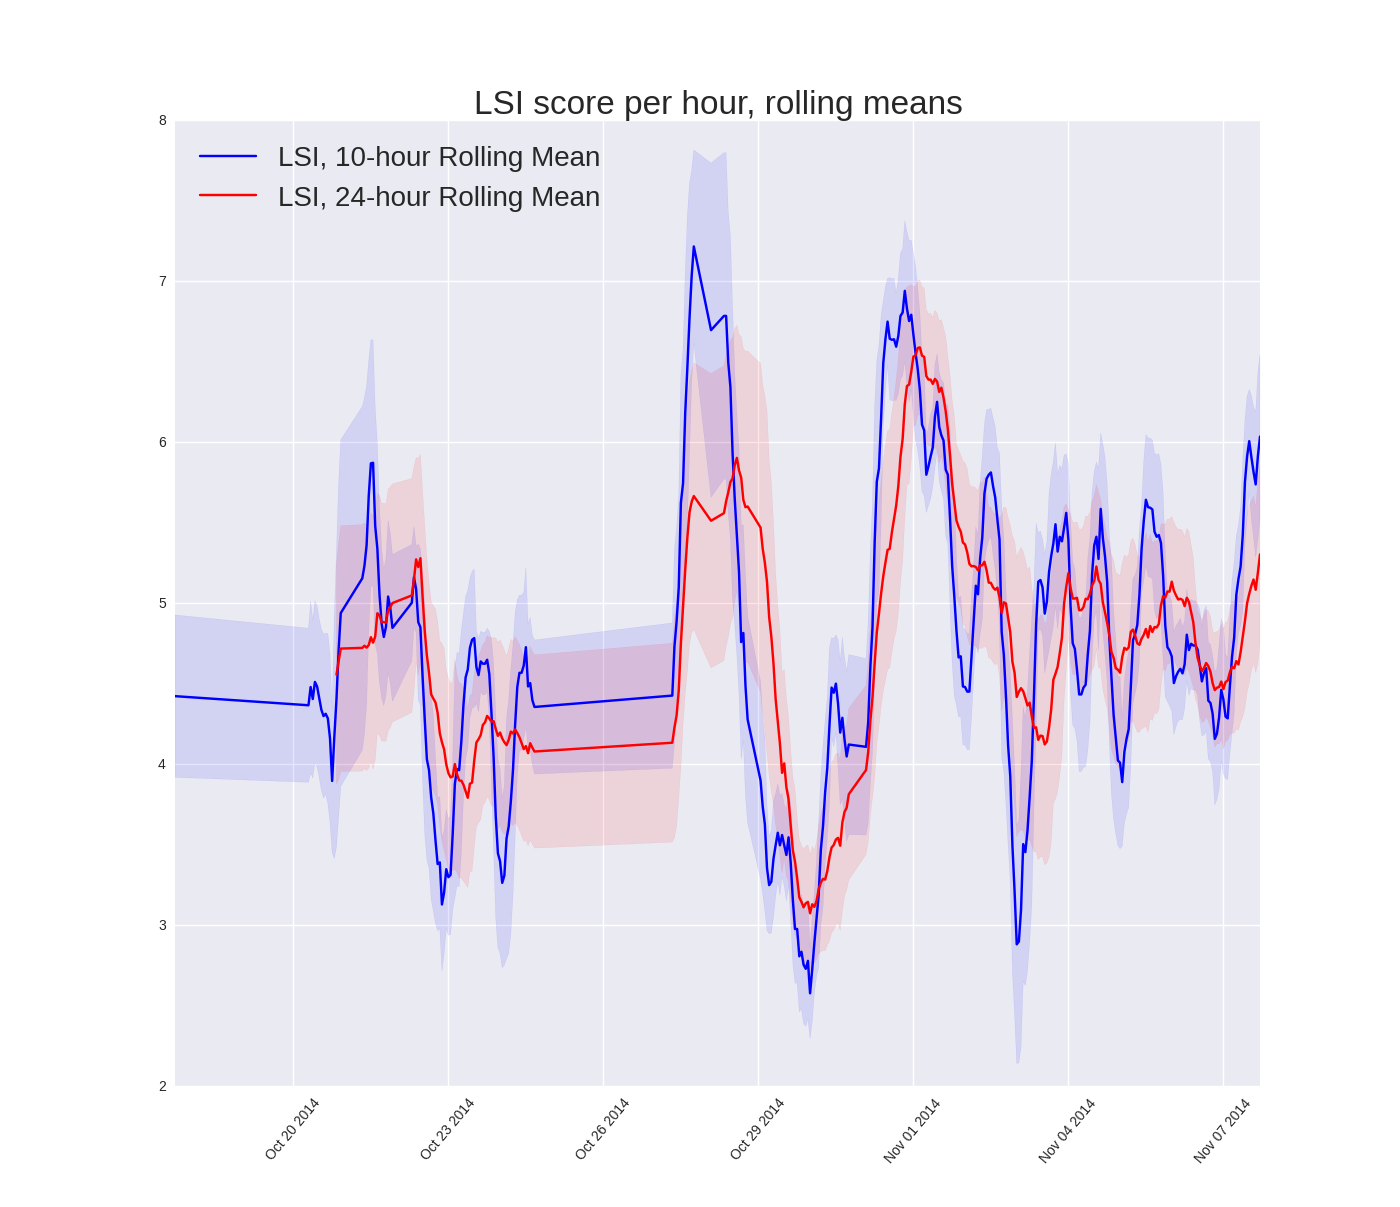
\includegraphics[width=4in]{figures/lsi_rolling_means.png}
               %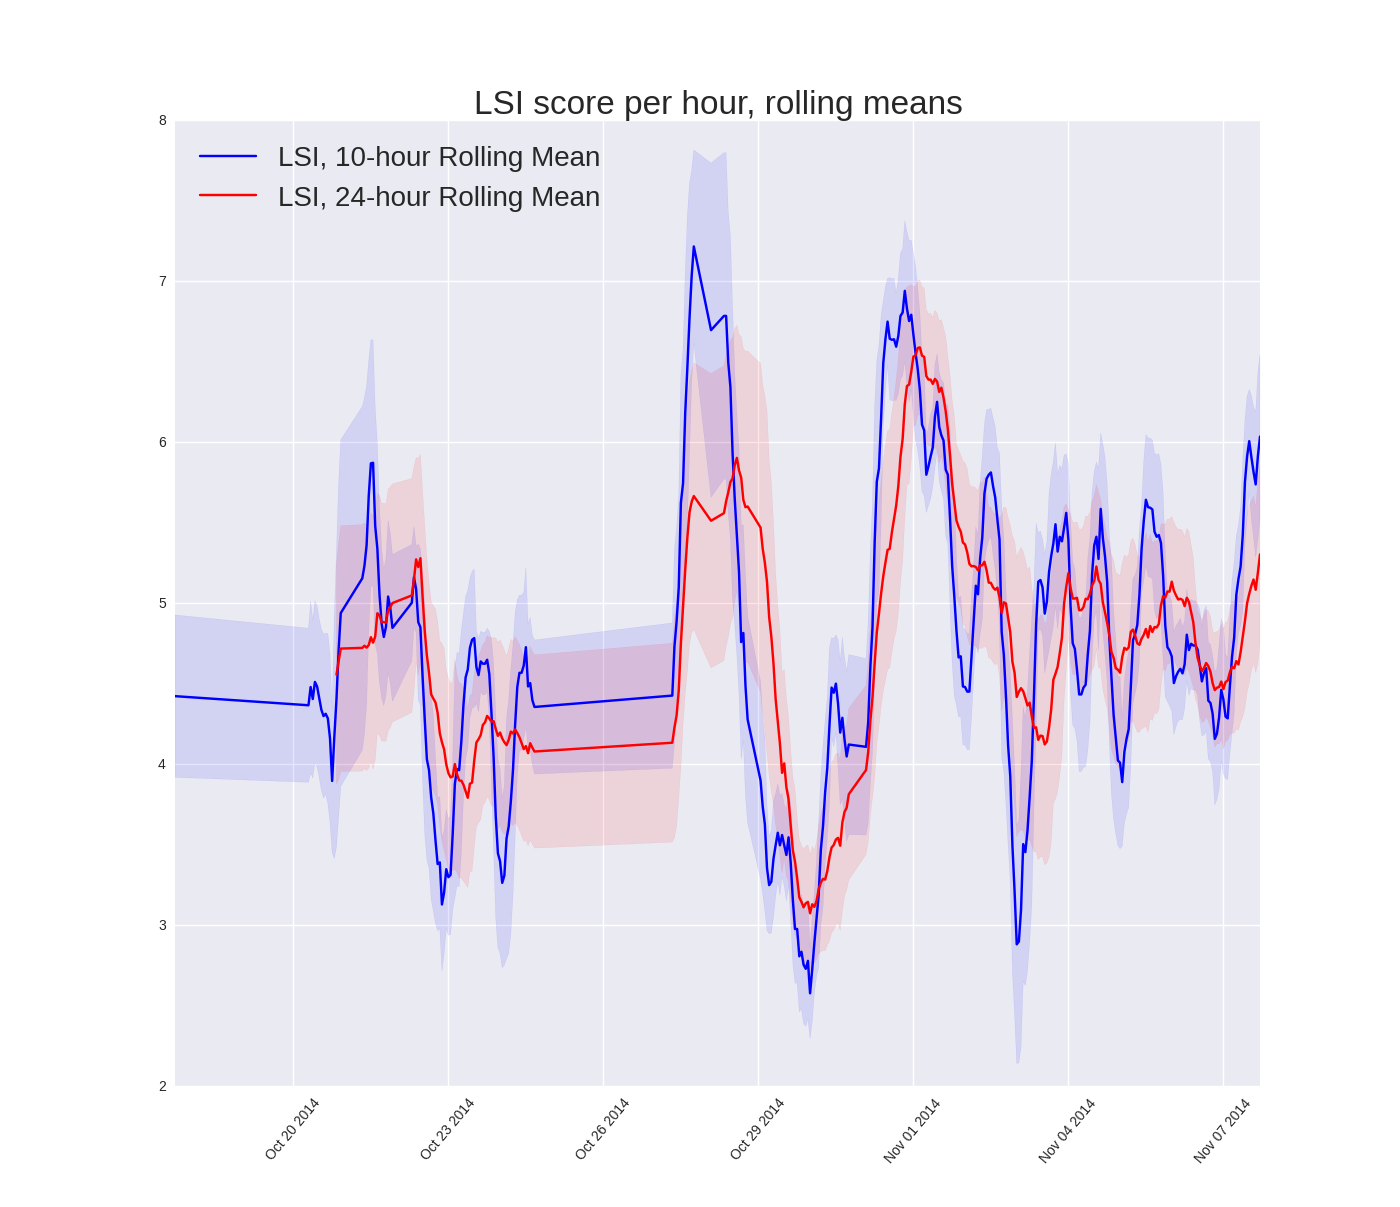
\includegraphics[width=0.99\linewidth]{figures/lsi_rolling_means.png}
             %\end{tikzfigure}
           %\end{wrapfigure}
           %\begin{itemize}
           %  \item Total tweets collected: 84 million
           %  \item Total hours analyzed: 218
           %%  \item Mean number of tweets per hour:
           %  \item Mean semantic score:  
           %\end{itemize}
           %\vspace{3cm}
           \begin{tikzfigure}[ Word cloud of LSI topics for time xxx ]
             \label{fig:wordcloud}
             {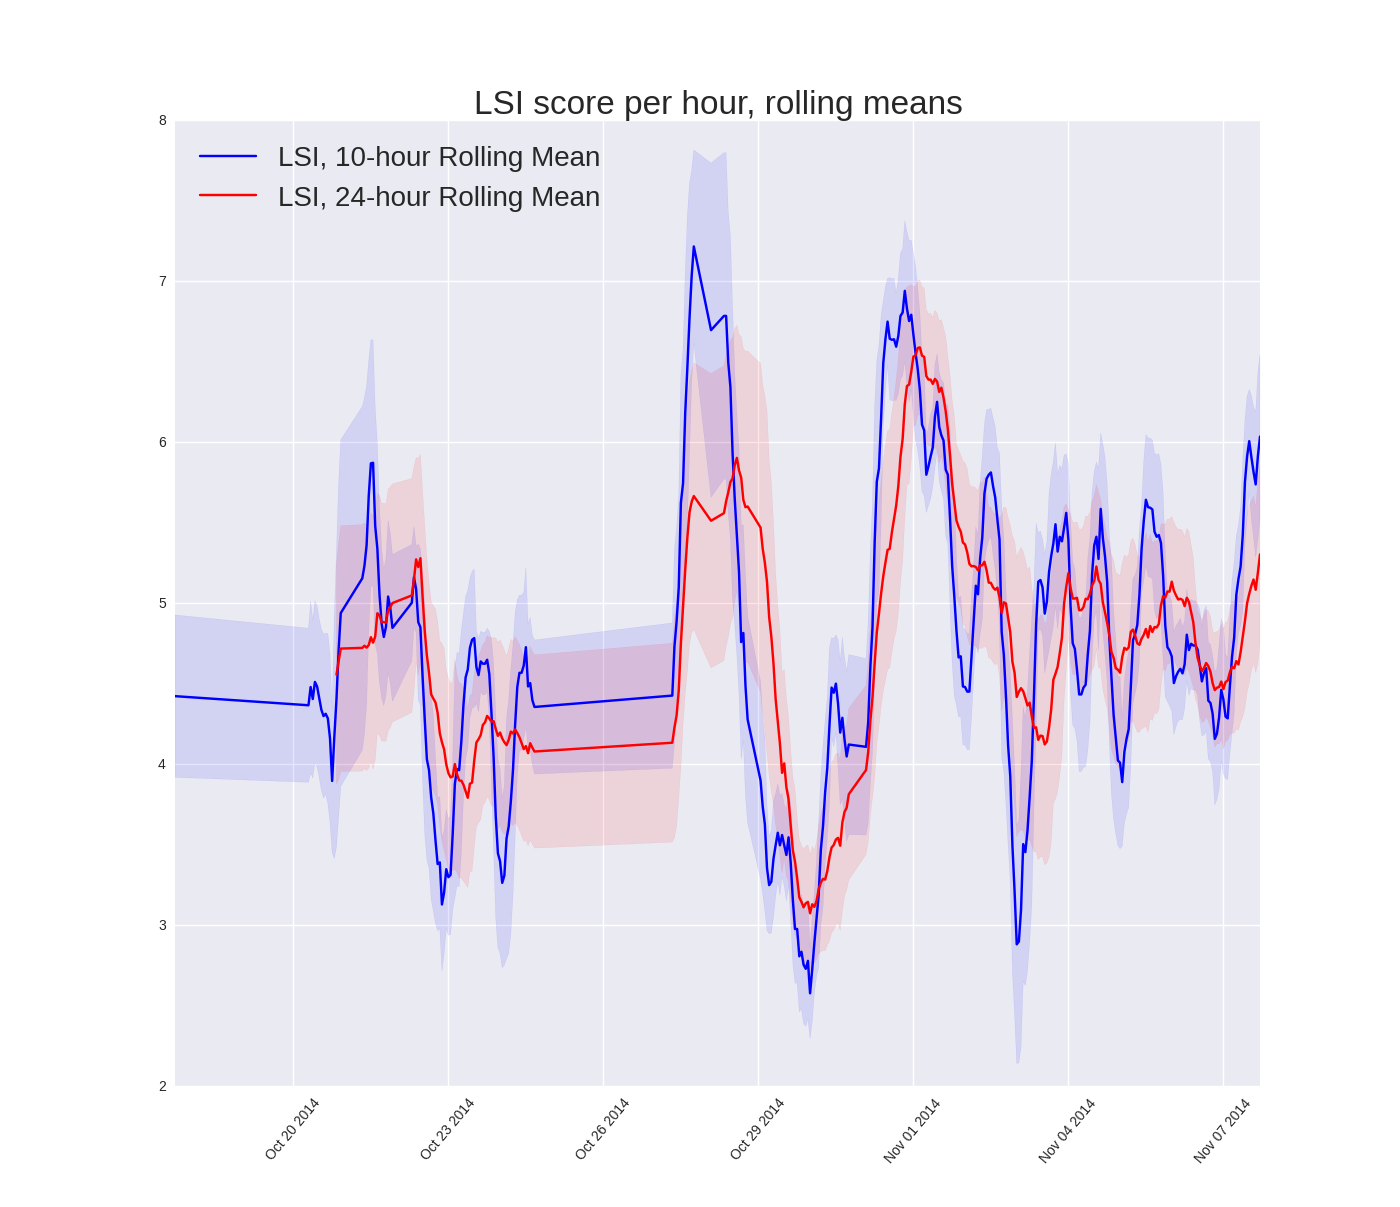
\includegraphics[width=0.46\linewidth]{figures/lsi_rolling_means.png}}
             {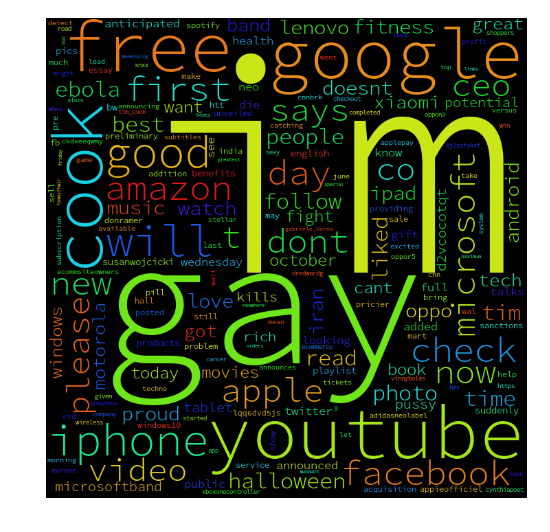
\includegraphics[width=0.35\linewidth]{../analysis/img170.png}}
             {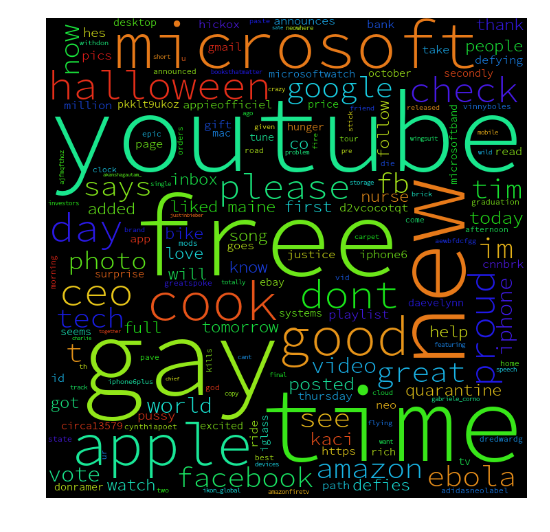
\includegraphics[width=0.35\linewidth]{../analysis/img173.png}}
           \end{tikzfigure}
         }

%%%%%%%%%%%%%%%%%%%%%%%%%%%%%%%%%%%%%%%%%%%%%%%%%%%%%%%%%%
%%%%%%%%%       new col         %%%%%%%%%%%%%%%%%%%%%%%%%%
%%%%%%%%%%%%%%%%%%%%%%%%%%%%%%%%%%%%%%%%%%%%%%%%%%%%%%%%%%

         \column{.5}
%%%%%%%%%%%%%%%%new block%%%%%%%%%%%%%%%%%%%%%%%%%%%%%%%%%%%%
         \block{Stocks}{
           \begin{tikzfigure}[Rolling means of LSI score per hour over
             sample.] \label{fig:means}
             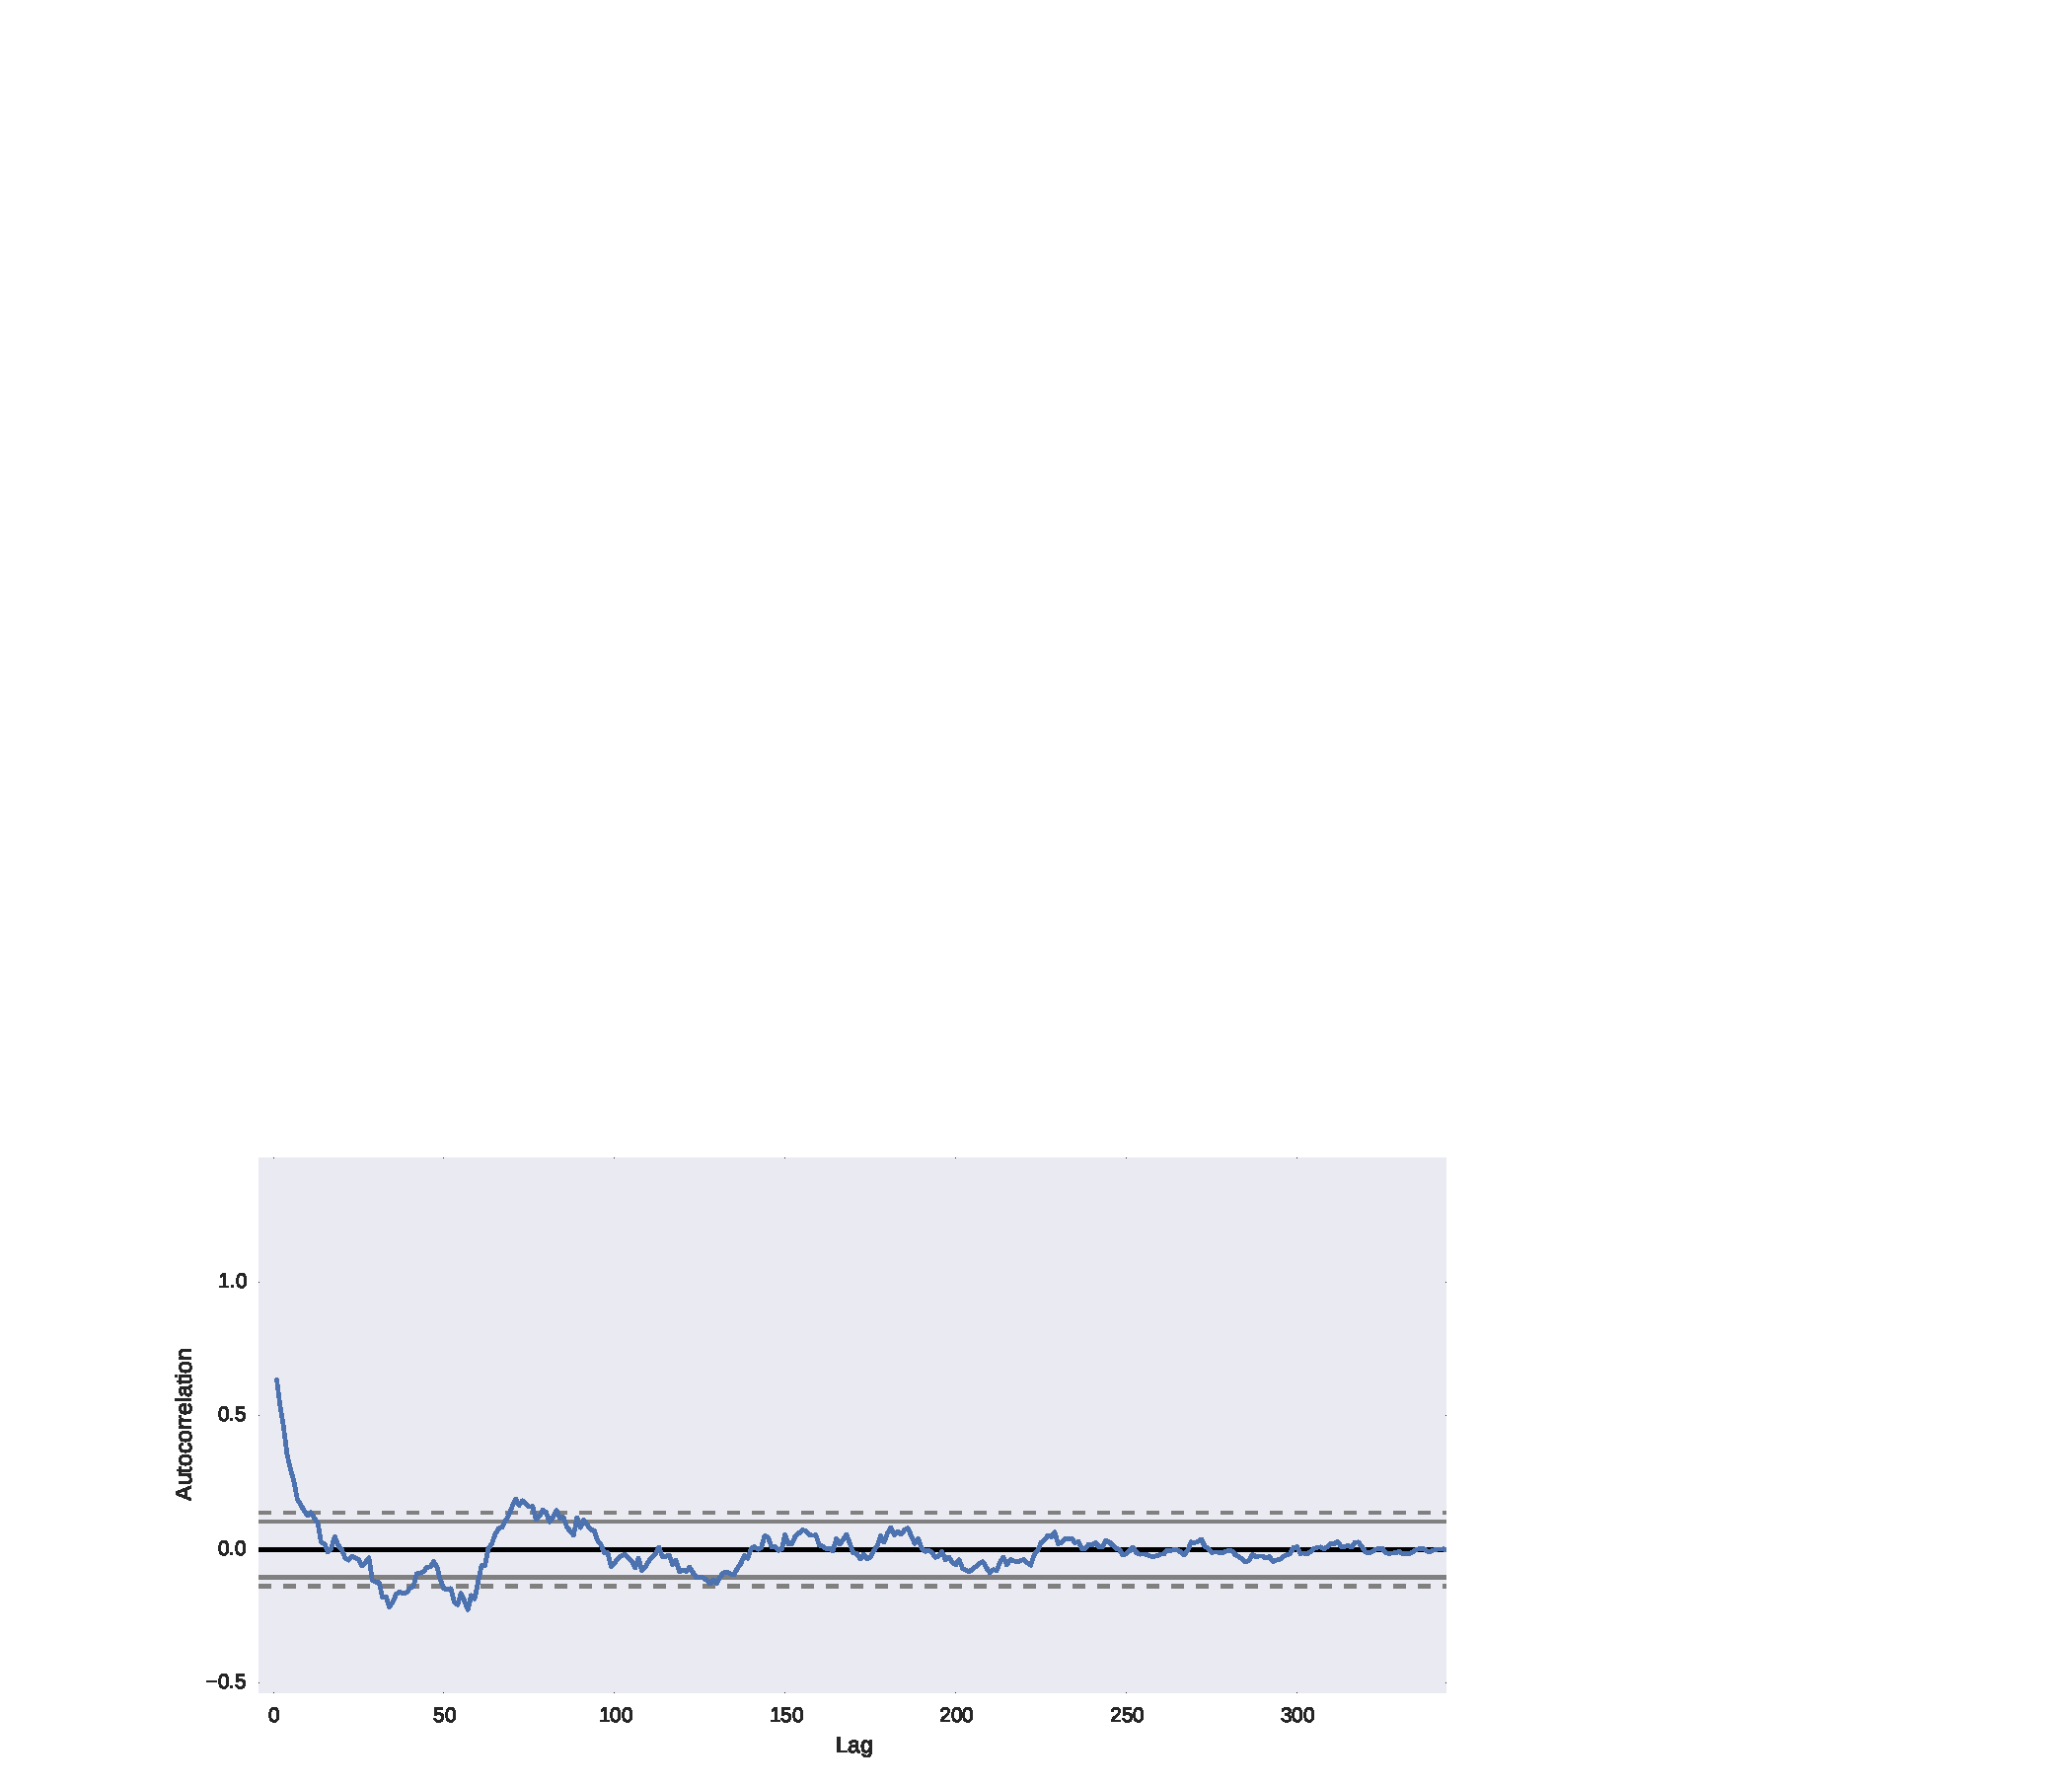
\includegraphics[width=7in]{figures/autocorr_plot.pdf}
           \end{tikzfigure}
         }
%%%%%%%%%%%%%%%%new block%%%%%%%%%%%%%%%%%%%%%%%%%%%%%%%%%%%%

   \block{VAR model results}{
    Vector Autoregression (VAR) models are used to model multivariate time
    series. They describe a set of $k$ variables as a linear function of
    their previous values. A $p$-th order VAR model is denoted by
    $y_t = c + A_1 y_{t-1} + A_2 y_{t-2} + \cdots + A_p y_{t-p} + e_t$
    A VAR model is often used with a lag operator that operates on the
    elements of a time series to produce the previous element. We determined
    the lag order by employing an information criteria-based order selection. 
   }

 \end{columns}


\end{document}




\endinput
%%
%% End of file `tikzposter-example.tex'.
